\documentclass{article}
\usepackage{arxiv}

\usepackage[utf8]{inputenc}
\usepackage[T1,T2A]{fontenc}
\usepackage[english, russian]{babel}   % use 8-bit T1 fonts
\usepackage{url}
\usepackage{booktabs}
\usepackage{amsfonts}
\usepackage{amsthm}
\usepackage{amssymb}
\usepackage{amsmath}
\usepackage{nicefrac}
\usepackage{microtype}
\usepackage{graphicx}
\usepackage{natbib}
\usepackage{doi}
\usepackage{algorithm}
\usepackage{algorithmic}

\newtheorem{theorem}{Теорема}
\newtheorem*{theorem-non}{Теорема}
\newtheorem{lemma}{Лемма}
\newtheorem*{lemma-non}{Лемма}
\newtheorem{assumption}{A}
\newtheorem*{assumption-non}{A}
\newtheorem{corollary}{Следствие}
\newtheorem*{corollary-non}{Следствие}
\DeclareMathOperator*{\argmax}{arg\,max}
\usepackage{subfig}
\DeclareMathOperator\supp{supp}


\usepackage{hyphenat}

\usepackage{comment} %comments
% Your figures are here:
\graphicspath{ {fig/} {../fig/} }


\title{Multiple learning in recommender systems}

\author{
	Nickolai Krekhov \\
	MIPT \\
        Dolgoprudny, Russia \\
        \texttt{krekhov.na@phystech.edu} \\
	%% examples of more authors
	\And
	Andrey Veprikov \\
	Department of Intelligent Systems
            \\MIPT\\Dolgoprudny, Russia\\\texttt{veprikov.as@phystech.edu}\\
	\And
	Anton Khritankov \\
        HSE University, MIPT\\
	Moscow, Russia\\
        \texttt{akhritankov@hse.ru}
}
\date{}


\hypersetup{
pdftitle={A template for the arxiv style},
pdfsubject={q-bio.NC, q-bio.QM},
pdfauthor={David S.~Hippocampus, Elias D.~Striatum},
pdfkeywords={First keyword, Second keyword, More},
}

\begin{document}
\maketitle

\begin{abstract}
        This paper addresses the issue of evaluating the quality of recommender systems in the long term, taking into account the evolution of consumers and product assortments. We consider the dynamical system of changes in consumers and products over time. The main purpose of the study is to identify the conditions under which degeneracies in audience, assortment, or transaction distribution occur in a given repeated machine learning system, and how such phenomena depend on the learning algorithms and recommendation models. Using the obtained results, we can present a model that is able to increase the metrics in the recommendation systems without degenerating the distributions on products and customers. We conduct a series of computational experiments on the synthetic datasets, the results of the experiments correspond to the theoretical predictions derived from the dynamical model
\end{abstract}


\keywords{Repeated Machine Learning \and Feedback loop}

\section{Introduction}
Here is an expanded introduction with more "glass on the water":

Recommender systems are an essential component of many online services, serving as powerful tools to offer users the most relevant and personalized content. These systems leverage various machine learning techniques to analyze user preferences, behaviors, and interactions, with the goal of providing tailored recommendations that enhance user experience and engagement. The widespread adoption of recommender systems across diverse domains, such as e-commerce, news platforms, and social networks, underscores their pivotal role in shaping modern digital experiences.

The importance of recommender systems is well-documented in numerous studies~[2, 3]. These systems have the ability to adapt to user preferences and interests, making them highly valuable for organizations seeking to improve customer satisfaction and drive revenue growth. However, the dynamic nature of recommender systems also introduces potential challenges, such as the emergence of "filter bubbles" and feedback loops that can lead to suboptimal results~[1, 4].

One particularly intriguing aspect of recommender systems is the phenomenon of multiple training, wherein data becomes available sequentially and is used to iteratively improve the system's predictive capabilities. This iterative learning process can have unexpected effects, potentially resulting in the degeneration of the distribution of original items~[5]. Addressing this issue is a crucial concern, as maintaining a diverse and representative item distribution is essential for providing users with a balanced and enriching recommendation experience.

Existing literature has explored various methods for optimizing recommendation metrics while ensuring the stability of distribution patterns over time. Researchers have approached the problem from different angles, such as addressing input data bias to improve algorithm performance~[8] and identifying sufficient conditions for when dynamic systems with multiple training can lead to distribution degeneration~[9]. However, a comprehensive mathematical model for the process of multiply learning in recommender systems has not been previously discussed in the literature.

In this article, we propose a novel mathematical model that aims to capture the dynamics of multiple training in recommender systems. Our primary goal is to develop an algorithm that can enhance known recommendation metrics, such as nDCG, RMM, and map@K~[6, 7], while simultaneously preventing the degeneration of user and item distributions. By addressing this critical challenge, we seek to contribute to the ongoing efforts to improve the reliability, fairness, and sustainability of recommender systems in the digital landscape.

\section{Постановка задачи}

Цель работы --- предложить алгоритм, который улучшает стандартные метрики для рекомендательных алгоримтов (p@K, map@K, nDCG, MRR) при условии, что не возникает вырождения распределения товаров и пользователей, или доказать, что такого не существует.

Покупатели $c$ и товары $w$ описываются конечным числом признаков, то есть $ \mathbf{c} \in C \subset \mathbb{R}^{d_c}, \mathbf{w} \in W \subset \mathbb{R}^{d_w}$.\\
На каждом шаге $t$ имеется совместное распределение: $(\mathbf{c}, \mathbf{w})^T \sim p^{t}_{c,w} (\mathbf{x_c} , \mathbf{x_w} )$ . Изменение этого распределения от шага $t$ к шагу $t + 1$ определяет оператор эволюции $\text{D}_t : \textbf{R}_{d_c + d_w} \rightarrow \textbf{R}_{d_c + d_w} $, где $R_n$ --- множество всех функций плотности на $\mathbb{R}^n:$
\begin{center}
$
        \mathbf{R_n} := \left\{f : \mathbb{R}^n \rightarrow \mathbb{R}_+ ~\text{and}~ \int\limits_{\mathbb{R}^n}f(x)dx = 1\right\}
        $
\end{center}

Таким образом, $p^{t + 1}(\mathbf{x_c}, \mathbf{x_w}) = \text{D}_t(p^{t})(\mathbf{x_c}, \mathbf{x_w})$.\\
\hspace*{10px}Введем функцию $u_{\text{true}}: \mathbb{R}^{d_c} \times \mathbb{R}^{d_w} \times \Omega_z \to \mathbb{R}$, которая для потребителя с признаками $\mathbf{x_c} \in \mathbb{R}^{d_c}$, товара с признаками $\mathbf{x_w} \in \mathbb{R}^{d_w}$ и каких-то неизвестных для нас признаков $x_z \in \Omega_z$ определяет истиную полезность. Чем больше значение функции $u_{\text{true}}$, тем более полезным считается товар для пользователя. Рекомендательному алгоритму неизвестны $x_z$, $\Omega_z$ и функция $u_{\text{true}}$. \\Функция $u_{\text{pred}}: \mathbb{R}^{d_c} \times \mathbb{R}^{d_w} \to \mathbb{R}$ --- оцененная рекомендательным алгоритмом функция полезности. \\
Рассмотрим множество сделок $F =  \left\{(c, w, u_{\text{true}}(c, w))^T | c, w \sim p_{c, w}(\mathbf{x_c}, \mathbf{x_w})\right\} \subseteq \mathbb{R}^{d_c + d_w + 1}$ и введем на нем функцию $p_u((\mathbf{x_c}, \mathbf{x_w}, u)^T) := u - u_{\text{pred}}(\mathbf{x_c}, \mathbf{x_w}) \in \mathbb{R} \\$
\hspace*{10px}Будем говорить, что распределение $p(x)$ вырождается, если

% $$ \mu(\supp p())$$
$$
\exists \phi(x) : \supp p(x) = \{x \; |\; \phi(x) = 0\}
$$

Введем функцонал качества:
            $$L^t(c, w) = \mathbb{E}_z[(u_{\text{true}}(c, w, z) - u_{\text{pred}}(c, w))^2],$$
Это означает, что $\phi(x)$ является уравнением поверхности меньшей размерности, которая и является носителем меньшей размерности.

Множеством вырождения будем называть $\Phi = \{x \; |\; \phi(x) = \inf\}$

Улучшение метрик означает, что должно происходить вырождение распределения на множестве $F$, однако тут в качестве $\phi$ мы возьмем конкретную функцию, а именно $p_u(x)$.

Итак, нужно предложить алгоритм, при использовании которого:
\begin{enumerate}
    \item $\neg \exists \phi(x) : \supp p_{c, w}^{\infty}(\mathbf{x_c}, \mathbf{x_w}) = \{x \; |\; \phi(x) = 0\}$
    \item $p_u^{\infty}((\mathbf{x_c}, \mathbf{x_w}, u)^T) = \delta(x)$, где $\delta(x)$ - дельта-функция Дирака
\end{enumerate}
или доказать, что такого не существует.

\subsection{Критерии качества модели}
Важным признаком для сравнения качества моделей является невырождение распределения $p^t_{c,w}$ пользователей-товаров.

\begin{enumerate}
    \item Вырождение распределения невязок: $u_{\text{true}} - u_{\text{pred}} \sim \delta(x)$, где $\delta(x)$ - дельта-функция Дирака.\\
    Условия такого вырождения описаны в статье [1], однако никаких гарантий на отсутствие выраждения $p^t_{c,w}$ нет.

    \item $y_{\text{true}} := Bern(u_{\text{true}})$,
    $y_{\text{pred}} := Bern(u_{\text{pred}})$\\
    Для каждого пользователя считаем $accuracy@K = \frac{\sum^K_{k = 1} (\mathbf{I}\{y^k_{\text{pred}} = y^k_{\text{true}}\})} {K}$ и затем усредняем по всем пользователям.

\end{enumerate}

\section{Основные результаты}
Для доказательства утверждений нужно сделать важное предположения о поведении пользователей и площадок с товарами.\\



{\bf Предположение 1}:
Функция интереса $u_{\text{true}}: \mathbb{R}^{d_c} \times \mathbb{R}^{d_w} \times \Omega_z \to \mathbb{R}$ существует.

{\bf Предположение 2}:
Пользователи и площадка с товарами ведут себя рационально, т.е. $p^{t+1}_{c, w}  \propto L^t(c, w)^{-1}$.
\\
\begin{theorem}

    \item Пусть выполнены Предположение 1 и Предположение 2. Тогда в зависимости от $u_{\text{pred}}$ множество $\Phi^t(x)$ будет иметь следующий вид:

    \begin{enumerate}

    \item $u^1_{\text{pred}}(c, w) = \mathbb{E}_z[(u_{\text{true}}(c, w, z)]$, \\
    % тогда $L^t(c, w) = \mathbb{D}_z[(u_{\text{true}}(c, w, z)]$\\
    $\Phi^t_1 = \left\{ (\mathbf{x_c}, \mathbf{x_w})^T \in \mathbb{R}^{d_c + d_w} \; | \; \mathbb{D}_z[(u_{\text{true}}(c, w, z)]=0 \; \right\}$\\


    \item
    $u^2_{\text{pred}}(c, w)$ =
    \begin{cases}
       1, &\text{$\mathbb{E}_z[(u_{\text{true}}(c, w, z)] \geq \frac{1}{2} $}\\
       0, &\text{иначе}
    \end{cases}, \\
    % $L^t(c, w) = \mathbb{D}_z[(u_{\text{true}}(c, w, z)] + \min \left(\mathbb{E}_z[(u_{\text{true}}(c, w, z)]^2; 1 -  \mathbb{E}_z[(u_{\text{true}}(c, w, z)]^2 \right)$\\

        $\Phi^t_2 = \left\{ (\mathbf{x_c}, \mathbf{x_w})^T \in \mathbb{R}^{d_c + d_w} \; | \; \text{для п.в. $x_z \in \Omega_z$ $u_{\text{true}}(c, w, z) = 1$ или 0 } \; \right\}$ \\

    \item  $u^3_{\text{pred}}(c, w) = a = const$, \\
    $\Phi^t_3 = \left\{ (\mathbf{x_c}, \mathbf{x_w})^T \in \mathbb{R}^{d_c + d_w} \; | \; \text{для п.в. $x_z \in \Omega_z$ $u_{\text{true}}(c, w, z) = a$} \; \right\}$ \\
    \end{enumerate}

\end{theorem}

Заметим, что выполнены вложения $\Phi^t_2 \subset \Phi^t_1$ и $\Phi^t_3 \subset \Phi^t_1$. Обратим внимание, что на точки, подходящие для $\Phi^t_2$ или $\Phi^t_3$ накладываются достаточно сильные ограничения. Это позволяет выдвинуть гипотезу, что вырождения при $u_{\text{pred}}(c, w) := u^2_{\text{pred}}(c, w)$ не будет, если $u_{\text{true}}$ почти всюду не равно 1 или 0.

\begin{lemma}
    \item Пусть $\xi, \eta$ - случайные величины, $\mathbb{P} \left\{0 \leq \xi,\eta \leq 1 \right\} = 1$,
    $\hat{\xi} \sim Bern(\xi)$, $\hat{\eta} \sim Bern(\eta)$ \\
    Тогда $\argmax_{\mathbb{E}[\eta]}\mathbb{P}\{|\hat{\xi} - \hat{\eta}| = 0\}$ =
    \begin{cases}
       1, &\text{$\mathbb{E}[\xi] \geq \frac{1}{2} $}\\
       0, &\text{иначе}
    \end{cases}
\end{lemma}

Если $\xi = u_{\text{true}}(c, w, z)$, а $\eta = u_{\text{pred}}(c, w)$, то согласно Лемме 1 $u_{\text{pred}}(c, w) := u^2_{\text{pred}}(c, w)$ из Теоремы 1 должен будет максимизировать метрику accuracy@K.

\section{Вычислительный эксперимент}
Целью эксперимента является проверка теоретических доказанных выше утвреждений. Мы проверим гипотезы о вырождении и не вырождении распределений в зависимости от функции $u_{\text{pred}}$ из Теоремы 1. Для этого мы будем считать дисперсию выборок товаров и пользователей на каждом шаге, а также строить графики и совместного распределения пользователей-товаров, и по отдельности. Также проверим выполнение леммы о том, что $u_{\text{pred}}(c, w)$ =
    \begin{cases}
       1, &\text{$\mathbb{E}_z[(u_{\text{true}}(c, w, z)] \geq \frac{1}{2} $}\\
       0, &\text{иначе}
    \end{cases} максимизирует метрику accuracy@K.
\subsection{Данные}
Данные используются синтетические, пользователи и товары имеют по одному параметру:
        $\\
        c \sim \mathcal{N}(0.6, 0.2), \qquad
        w \sim \mathcal{N}(0, 0.4),  \qquad
        z_t \sim \mathcal{N}(0, \frac{0.05}{t}),  \qquad
        $\\
    Эксперимент будет проводиться для двух функций $u_{\text{true}}(c,w,z)$.


\subsection{Описание эксперимента}
В качестве алгоритма рекомендаций, оценивающего $u_{\text{true}}$, будем использовать нейронную сеть.
Будем запускать динамическую во времени систему на 100 итераций. Одна итерация выглядит следующим образом:
\begin{enumerate}
\item Происходит сэмплирование выборок произвольного размера покупателей и товаров из распределений $f_c^t$ и $f_w^t$:
$c_1^t,..,c_n^t \sim f_c^t,\ w_1^t,..,w_k^t \sim f_w^t$.
\item Рекомендательная система подбирает для каждого покупателя из выборки подмножество товаров из $w_1^t,..,w_k^t$
\item Покупатели совершают покупку с вероятностью $u_{\text{true}}(c, w, z)$ Далее рекоммендательная система дообучается на полученном фидбэке, используя базовый алгоритм рекомендательный системы.
\item Шаги 2-3 повторяются произвольное количество раз.
\item Далее проиходит обновление распределений товаров и пользователей в соответствии со значениями функции $L$ в точках  $(c, w)$, $c \in \{ c_1^t,..,c_n^t \}, \; w \in \{ w_1^t,..,w_k^t \}$ . Будем это делать при помощи ядерной оценки плотности.
\end{enumerate}

Будем рассматривать следующие функции полезности:
\begin{enumerate}
\item $u_{\text{true}}(c, w, z) = \frac{\arctan(c - w + z)}{\pi} + 0.5$ \\
Ожидаем, что распределния будут сдвигаться, так как чем больше значение $c-w$, тем более вероятна покупка, поэтому ожидается, что математическое ожидание признака пользователя будет увеличиваться, а признака предетов уменьшаться.
\item$u_{\text{true}}(c, w, z) = \exp{(-0.5((c - c_0)^2 + (c - w_0)^2 + z^2))}, c_0 = 1, w_0 = 0.2 $\\
Ожидаем, что распределния будут вырождаться в точке $(c_0, w_0)$, так как в ней достигается наибольшее значение функции полезности.
\end{enumerate}


\begin{figure}[h!]
    \centering
    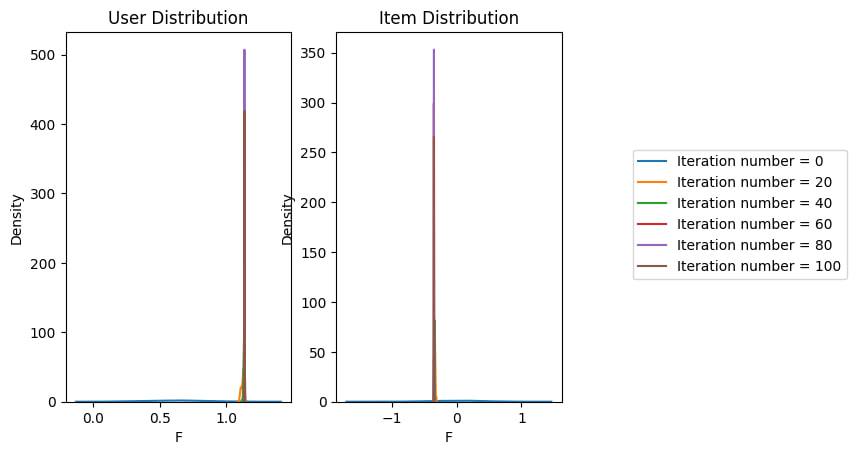
\includegraphics[width=0.49\linewidth]{images/distr_utrue1.jpg}
    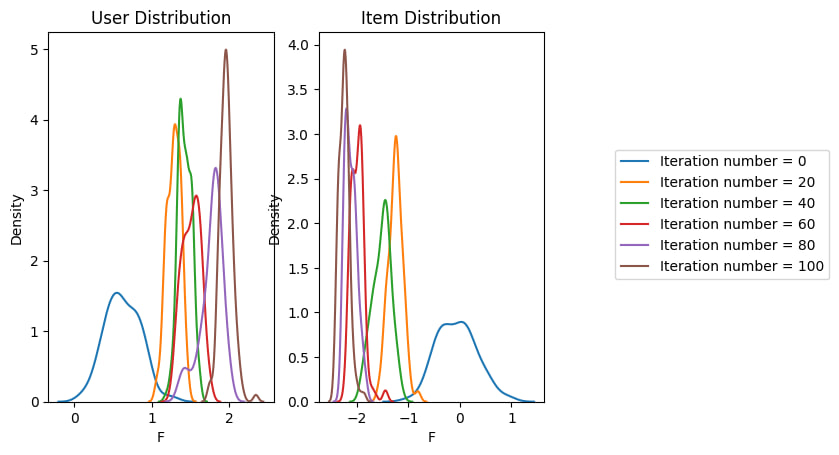
\includegraphics[width=0.49\linewidth]{images/distr_utrue1_2.jpg}

    \caption{Распределения после 100 итераций. case 1 (left), case 2 (right) \\
    $u_{\text{true}}(c, w, z) = \frac{\arctan(c - w + z)}{\pi} + 0.5$}
    \label{distribtopns}
\end{figure}




\subsection{Результаты эксперимента}
\begin{enumerate}
    \item На Рис. 1 показаны распределения на конкретных итерациях. Как и ожидалось, для $u_{\text{pred}}$ из первого пункта Теоремы 1 происходит вырождение, а для функции из второго пункта вырождения нет. Причем во обеих случаях мат. ожижание дейстивтельно имело тренд смещения таким образом, чтобы значение $c-w$ увеличилось. \\
    Теперь посмотрим на значения функции $L(c, w)$ и метрики accuracy@4.
    Видим, что в случае case 2 значение метрики accuracy@4 больше чем в case 1, что соответсвует полученным нами теоретическим результатам в Лемме 1: $u_{\text{pred}} = \begin{cases}
       1, &\text{$\mathbb{E}_z[(u_{\text{true}}(c, w, z)] \geq \frac{1}{2} $}\\
       0, &\text{иначе}
    \end{cases}$ максимизирует accuracy@k . Однако значение функции L меньше в case 1, это говорит о том, что вырождение происходит намного быстрее в case 1. Еще это говорит о том, что в case 1 алгоритм более точно предсказывает $u_{\text{true}}$, а то, что accuracy@4 меньше объясняется тем, что в носителе распределения уже отсутсвуют значения $c, w$, на которых может достигаться большее значение $u_{\text{pred}}$.
\end{enumerate}


\begin{figure}[h!]
    \centering
    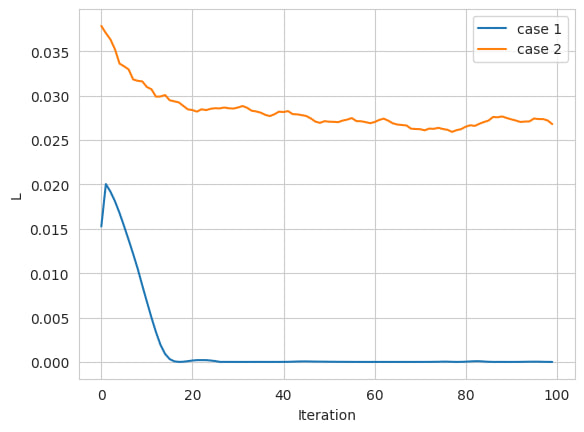
\includegraphics[width=0.49\linewidth]{images/loss.jpg}
    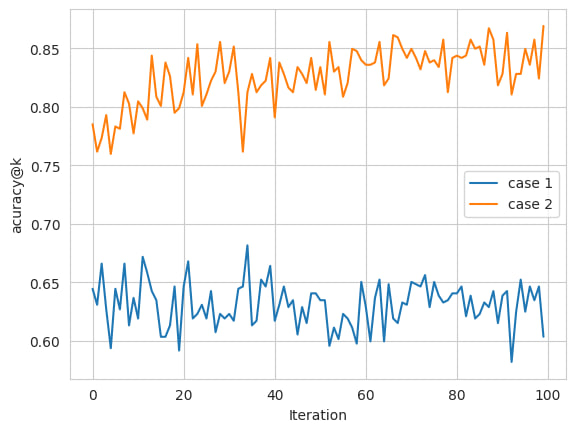
\includegraphics[width=0.49\linewidth]{images/case1_csae2.jpg}

    \caption{Значение функции L (слева), accuracy@4 (справа) в зависимости от номера итерации \\
    $u_{\text{true}}(c, w, z) = \frac{\arctan(c - w + z)}{\pi} + 0.5$}
    \label{accuracis}
\end{figure}

% \begin{figure}
%     \centering
%     \begin{subfigure}{0.6\textwidth}
%         \centering
%         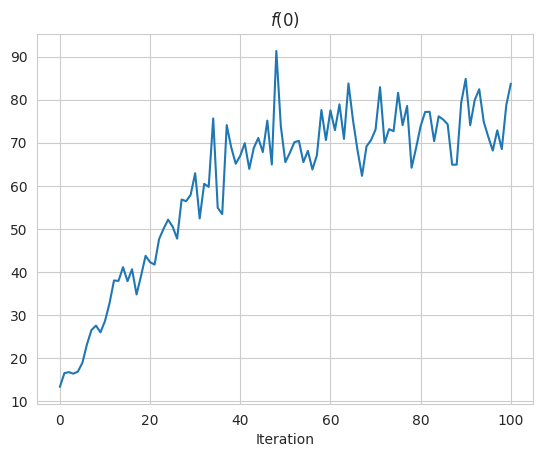
\includegraphics[width=0.8\linewidth]{images/f0.png}
%         \caption{$p_u(0)$}
%         \label{fig:p0}
%     \end{subfigure}%
%     \begin{subfigure}{0.6\textwidth}
%         \centering
%         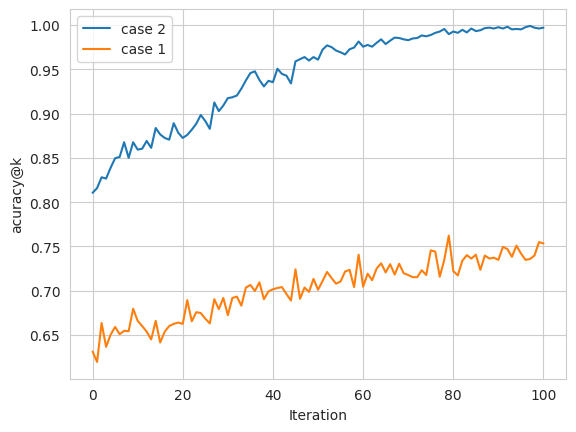
\includegraphics[width=0.8\linewidth]{images/accuracyk.png}
%         \caption{accuracy@K}
%     \end{subfigure}
%     \caption{Значения метрик от номера итерации}
%     \label{fig:two_images}
% \end{figure}


% \begin{figure}
%     \centering
%     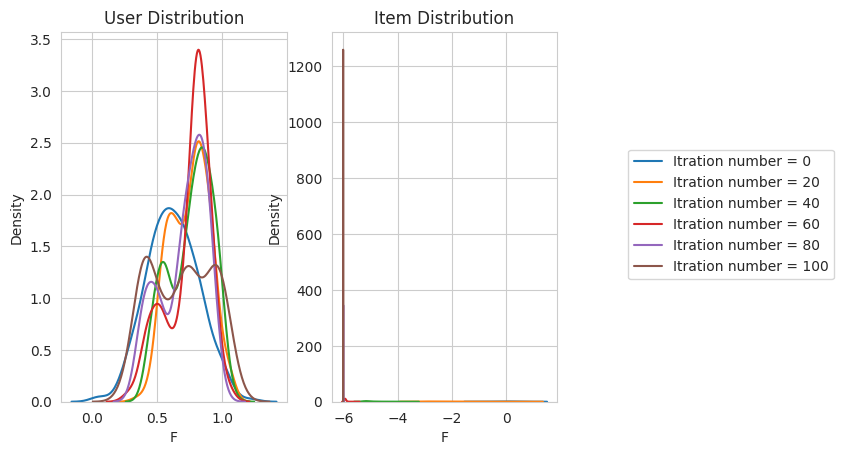
\includegraphics[width=0.8\textwidth]{images/distrChang2.png}
%     \caption{Распределение фичей пользователей и товаров в зависимоти от номер итерации}
%     \label{fig:distr}
% \end{figure}


% Теперь эксперимент, когда вырождение отсутствует:


% \begin{figure}

%     \centering
%     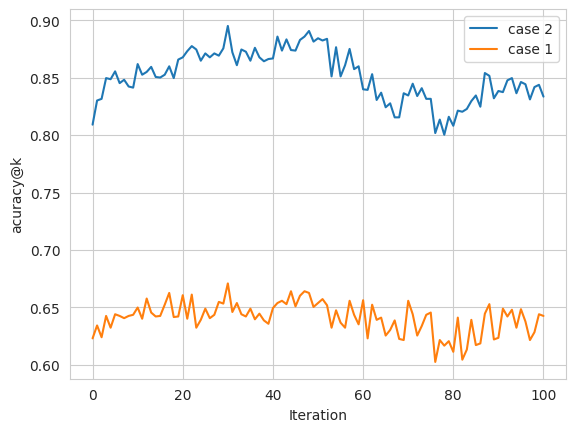
\includegraphics[width=0.5\textwidth]{images/noDegacc.png}
%     \caption{$p_u(0)$}
%     \label{fig:p1}

% \end{figure}


% \begin{figure}
%     \centering
%     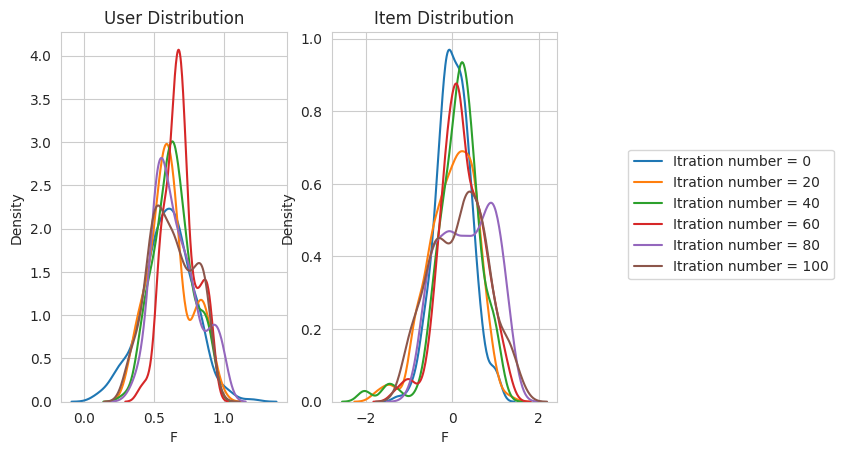
\includegraphics[width=0.8\textwidth]{images/noDeg.png}
%     \caption{Распределение фичей пользователей и товаров в зависимоти от номер итерации}
%     \label{fig:distr1}
% \end{figure}

\section{Заключение}
TODO


\newpage
\bibliographystyle{unsrtnat}
\bibliography{References}

[1] Dominic Spohr. Fake news and ideological polarization: Filter bubbles and selective exposure on social media. \newline
[2] Billsus, Daniel & Pazzani, Michael. (2003). User Modeling for Adaptive News Access. User Modelling and User-Adapted Interaction. 10. 10.1023/A:1026501525781.\newline
[3] Pedreschi, D. and Miliou, I. and European Parliament. Directorate-General for Internal Policies of the Union Artificial Intelligence (AI): new developments and innovations applied to e-commerce European Parliament, 2020.\newline
[4] Krauth K., Wang Y., Jordan M. I. Breaking feedback loops in recommender systems with causal inference //arXiv preprint arXiv:2207.01616. – 2022.\newline
[5] Khritankov, Anton. 2023. “Positive Feedback Loops Lead to Concept Drift in Machine Learning Systems.” Applied Intelligence 53 (19): 22648–66. https://doi.org/10.1007/s10489-023-04615-3.\newline
[6] Yongfeng Zhang, Xu Chen, Qingyao Ai, Liu Yang, and W. Bruce Croft. 2018. Towards Conversational Search and Recommendation: System Ask, User Respond. In Proceedings of the 27th ACM International Conference on Information and Knowledge Management (CIKM '18). Association for Computing Machinery, New York, NY, USA, 177–186. https://doi.org/10.1145/3269206.3271776\newline
[7] Wang, Y., Wang, L., Li, Y., He, D. &amp; Liu, T.. (2013). A Theoretical Analysis of NDCG Type Ranking Measures. <i>Proceedings of the 26th Annual Conference on Learning Theory</i>, in <i>Proceedings of Machine Learning Research</i> 30:25-54 Available from https://proceedings.mlr.press/v30/Wang13.html.\newline
[8] Krueger, D., Maharaj, T., & Leike, J. (2020). Hidden incentives for auto-induced distributional shift. arXiv preprint arXiv:2009.09153.
[9] Burtini, Giuseppe & Loeppky, Jason & Lawrence, Ramon. (2015). Improving Online Marketing Experiments with Drifting Multi-Armed Bandits. ICEIS 2015 - 17th International Conference on Enterprise Information Systems, Proceedings. 1. 10.5220/0005458706300636.


\newpage
\begin{center}
    \LARGE \textbf{Appendix}
\end{center}
\normalsize

\appendix

        \section{Proof of theorem}
    \begin{proof}

        $L^t(c, w) = \mathbb{E}_z[(u_{\text{true}}(c, w, z) - u_{\text{pred}}(c, w))^2]$ переписывается в виде:
        $L^t(c, w) = \mathbb{D}_z[(u_{\text{true}}(c, w, z)] + \left(\mathbb{E}_z[(u_{\text{true}}(c, w, z)] - u_{\text{pred}}(c, w)\right)^2$, так как
        $L^t(\mathbf{x_c}, \mathbf{x_w}) = \mathbb{E}_z \left[(u_{\text{true}}(\mathbf{x_c}, \mathbf{x_w}, x_z)-u_{\text{pred}})^2 \right] = \mathbb{E}_z \left[(u_{\text{true}}(\mathbf{x_c}, \mathbf{x_w}, x_z) -  \mathbb{E}_z \left[  u_{\text{true}}(\mathbf{x_c}, \mathbf{x_w}, x_z) \right] + \mathbb{E}_z \left[ u_{\text{true}}(\mathbf{x_c}, \mathbf{x_w}, x_z) \right] - u_{\text{pred}}(\mathbf{x_c}, \mathbf{x_w}))^2 \right] = \mathbb{E}_z \left[(u_{\text{true}}(\mathbf{x_c}, \mathbf{x_w}, x_z) -  \mathbb{E}_z \left[  u_{\text{true}}(\mathbf{x_c}, \mathbf{x_w}, x_z) \right])^2\right] + \mathbb{E}_z \left[( \mathbb{E}_z \left[  u_{\text{true}}(\mathbf{x_c}, \mathbf{x_w}, x_z) \right] -  u_{\text{pred}}(\mathbf{x_c}, \mathbf{x_w}))^2\right]  + 2\mathbb{E}_z \left[u_{\text{true}}(\mathbf{x_c}, \mathbf{x_w}, x_z) -  \mathbb{E}_z \left[  u_{\text{true}}(\mathbf{x_c}, \mathbf{x_w}, x_z) \right]\right] \cdot  (\mathbb{E}_z \left[ u_{\text{true}}(\mathbf{x_c}, \mathbf{x_w}, x_z) \right] - u_{\text{pred}}(\mathbf{x_c}, \mathbf{x_w})) = \mathbb{D}_z \left[ u_{\text{true}}\right] + ( \mathbb{E}_z \left[  u_{\text{true}}(\mathbf{x_c}, \mathbf{x_w}, x_z) \right] -  u_{\text{pred}}(\mathbf{x_c}, \mathbf{x_w}))^2 $, так как $$\mathbb{E}_z \left[u_{\text{true}}(\mathbf{x_c}, \mathbf{x_w}, x_z) -  \mathbb{E}_z \left[  u_{\text{true}}(\mathbf{x_c}, \mathbf{x_w}, x_z) \right]\right] = 0$$.

    \end{proof}



    \section{Proof of Lemma}
    Пусть $\xi, \eta$ - случайные величины, $\mathbb{P} \left\{0 \leq \xi,\eta \leq 1 \right\} = 1$,
    $\hat{\xi} \sim Bern(\xi)$, $\hat{\eta} \sim Bern(\eta)$ \\
    Тогда $\argmax_{\mathbb{E}[\eta]}\mathbb{P}\{|\hat{\xi} - \hat{\eta}| = 0\}$ =
    \begin{cases}
       1, &\text{$\mathbb{E}[\xi] \geq \frac{1}{2} $}\\
       0, &\text{иначе}
    \end{cases}
    $
    \begin{proof}

    Заметим, что
    $\mathbb{E}[\xi] = 1 \cdot \mathbb{P}\{\xi = 1\} + 0 \cdot \mathbb{P}\{\xi = 0\} = \mathbb{P}\{\xi = 1\}$
    $\mathbb{P}\{\xi = 0\} = 1 - \mathbb{E}[\xi]$

    $\mathbb{P}\{|\hat{\xi} - \hat{\eta}| = 0\} = \mathbb{P}\{\hat{\xi} = \hat{\eta}\} = \mathbb{P}\{\xi = 1\} \mathbb{P}\{\eta = 1\} + \mathbb{P}\{\xi = 0\}\mathbb{P}\{\eta = 0\} = \mathbb{E}[\xi] \mathbb{E}[\eta] + (1 - \mathbb{E}[\xi])(1 - \mathbb{E}[\eta])$
    Это линейная функция от $\mathbb{E}[\eta]$, следовательно ее максимум достигается на на одном из концов, т.е.
    $\max_{\mathbb{E}[\eta]}(\mathbb{E}[\xi] \mathbb{E}[\eta] + (1 - \mathbb{E}[\xi])(1 - \mathbb{E}[\eta])) = \max\{\mathbb{E}[\xi], 1 - \mathbb{E}[\xi]\}$



    \end{proof}


\end{document}


